\documentclass[handout]{beamer}
\usepackage{graphicx,hyperref,color,epsfig}
\usepackage[UKenglish]{babel}
\usefonttheme[onlymath]{serif}

\mode<presentation>
%\usetheme{default} %Boadilla Singapore Warsaw
\usetheme{Boadilla}
%\setbeamercovered{transparent} %
\setbeamertemplate{itemize item}{$\bullet$} %
\setbeamertemplate{itemize subitem}{--} %
\setbeamertemplate{navigation symbols}{}

\newcommand{\pd}[1]{\parbox[c]{0.6 cm}{\fontsize{8}{8} \selectfont \centering #1}}
\newcommand{\ps}[1]{\parbox[c]{1 cm}{\fontsize{8}{8} \selectfont \centering #1}}
\newcommand{\pc}[1]{\parbox[c]{1 cm}{\fontsize{8}{8} \selectfont \centering #1}}
\newcommand{\pr}[1]{\parbox[c]{10 cm}{\fontsize{8}{8} \selectfont \centering #1}}
\newcommand{\pf}[1]{\parbox[l]{4.5 in}{\fontsize{5}{5} \selectfont #1}}
\newcommand{\pBig}[1]{\parbox[l]{4.5 in}{\fontsize{10}{10} \selectfont #1}}

%\title[\fontsize{4}{4} \selectfont MC and WinBUGS]{\fontsize{15}{15} \selectfont Introduction to monte Carlo methods and WinBUGS}
\date[\fontsize{4}{4} \selectfont MSc in Modern Epidemiology]{}
\author[\fontsize{4}{4} \selectfont Marta Blangiardo]{}

\institute[\fontsize{4}{4} \selectfont Imperial
College]{}

\begin{document}
%\frame{\titlepage}
\frame{
\begin{center}
\textbf{\Large Lecture 9.\\ Hierarchical Regression Models}\\
\end{center}
}

%%%%%%%%%%%%%%%%%%%%%%%%%%%%%%%%%%%%%%%%%%%%%%%%%%%%%%%%%%%%%%
\frame{\frametitle{Learning Outcomes}
After this session students should be able to:
\begin{itemize}
  \item Explain how a hierarchical structure can be applied to regression models;
  \item Describe how hierarchical models can be extended to include more than two levels and cross-classified data;
  \item Use hierarchical models for modelling variances.
\end{itemize}
}
%%%%%%%%%%%%%%%%%%%%%%%%%
\frame{
\frametitle{Hierarchical regression models}
\begin{itemize}
  \item Hierarchical structure can be applied to regression models
  \item One intercept and/or slope for each group (e.g. individual) which are then exchangeable
\end{itemize}

\pause\vspace{0.5cm}{\bf e.g. linear regression}
\begin{itemize}
\item $i=1,\ldots, I_j$ groups, $j=1,\ldots,J$ measurements

$\rightsquigarrow y_{ij} \sim N(\mu_{ij},\sigma^2) \hspace{1cm}  \mu_{ij} = \alpha_i + \beta_i x_{ij}$
\end{itemize}

\vspace{-2cm}\begin{tabular}{ccc}
\begin{minipage}{3cm}
\vspace{3cm}\fontsize{7}{7}\selectfont{$y_{ij}\sim N(\alpha_i + \beta x_{ij}, \sigma^2)$\\
$\alpha_i\sim N(m_{\alpha},s^2_{\alpha})$\\
$\beta \sim N(0,10000)$}
\end{minipage}

& \scalebox{0.25}{\rotatebox{270}{\includegraphics{figs/HierarcReg.eps}}}

&

\begin{minipage}{3cm}
\vspace{3cm}\fontsize{7}{7}\selectfont{$y_{ij} \sim N(\alpha_i + \beta_i x_{ij}, \sigma^2)$\\
$\alpha_i \sim N(m_{\alpha},s^2_{\alpha})$\\
$\beta_i \sim N(m_{\beta},s^2_{\beta})$}
\end{minipage}

\end{tabular}
}

%%%%%%%%%%%%%%%%%%%%%%%%%%%%%%%%%%%%%%%%%%%%%%%%%%%%%%%%%%%%%%
\frame{
\frametitle{Example: Hepatitis B Immunisation}

{\it Background}

\vspace{-.2cm}

\begin{itemize}
   \item Hepatitis B (HB) is endemic in Africa
   \item National program of childhood vaccination against HB introduced in Gambia
   \item Program effectiveness depends on duration of immunity afforded by vaccination    \end{itemize}

\vspace{-0.2cm}

\pause{\it Data}

\vspace{-.2cm}

   \begin{itemize}
   \item 106 children immunized against HB
   \item For each child: anti-HB titre measured at time of vaccination (baseline) and on 2 or 3 follow-up occasions
\end{itemize}
\vspace{-0.2cm}

\pause{\it Study objective}

\vspace{-.2cm}

   \begin{itemize}
   \item To obtain a model useful for predicting an individual child's protection against HB after vaccination
   \end{itemize}

\vspace{-0.2cm}

\pause{\it Related studies}

\vspace{-.2cm}

   \begin{itemize}
   \item Similar study in Senegal found:
   $$\hbox{anti-HB titre}  \propto  \frac{1}{T} $$
   where $T$ = time since HB vaccination
   \end{itemize}
}
%%%%%%%%%%%%%%%%%%%%%%%%%%%%%%%%%%%%%%%%%%%%%%%%%%%%%%
\frame{

Raw data for a subset of 106 individuals
\begin{center}
\scalebox{0.5}{
\includegraphics[bb=36 234 577 569]{figs/hep.raw.ps}}
\end{center}
}
%%%%%%%%%%%%%%%%%%%%%%%%%%%%%%%%%%%%%%%%%%%%%%%%%%%%%%%%%%
\frame{
\frametitle{Non hierarchical linear model (LM) for the HB data}
\begin{itemize}
\item[1.] Probability distribution(likelihood) for responses:
\begin{eqnarray*}
y_{ij} & \sim & \hbox{Normal}(\mu_{ij}, \sigma^2)
\end{eqnarray*}
where $y_{ij}$ = log of the $j$th anti-HB titre measurement for child $i$ \\
\pause\item[2.] Linear predictor:
\begin{eqnarray*}
\mu_{ij} = \alpha + \beta (t_{ij} - \overline{t}) + \gamma (y_{0i} -
\overline{y_0})
\end{eqnarray*}
where
\begin{itemize}
\item[] $t_{ij}$ = log of time (days since
vaccination) of $j$th measurement\\ for child $i$
\item[] $y_{0i}$ = log of baseline anti-HB titre for child $i$ \\
\end{itemize}
\end{itemize}

\pause{\bf Problems}
\begin{itemize}
\item Assumes a common regression line for all children
\item Takes no account of the repeated measurements within children
\end{itemize}
}
%%%%%%%%%%%%%%%%%%%%%%%%%%%%%%%%%%%%%%%%%%%%%%%%%%%%%%%%%%%%%%%%%%%%
\frame{
\begin{small}
\begin{itemize}
  \item[$\Rightarrow$] modify LM to allow separate intercept and slope for each child:
\begin{eqnarray*}
y_{ij} & \sim & \hbox{Normal}(\mu_{ij}, \sigma^2) \\
\mu_{ij}  & = & \alpha_i + \beta_i (t_{ij} - \overline{t}) + \gamma
(y_{0i} - \overline{y_0})
\end{eqnarray*}
Assumes that {\it conditionally} on $\alpha_i$ and $\beta_i$,
$\{y_{ij}, j= 1, 2,..  \}$ are independent
\pause\item Assume $\alpha_i$'s are exchangeable and
$\beta_i$'s are exchangeable, e.g.
\begin{eqnarray*}
\alpha_i & \sim & \hbox{Normal}(\mu_{\alpha}, \sigma^2_{\alpha}) \;\;\;\; i=1,...,106  \\
\beta_i & \sim & \hbox{Normal}(\mu_{\beta}, \sigma^2_{\beta})
\;\;\;\; i=1,...,106
\end{eqnarray*}

\pause\item We may then assume vague priors for the {\it
hyperparameters} of the population distribution, e.g.
\begin{eqnarray*}
\mu_{\beta}, \mu_{\alpha} & \sim & \hbox{Normal}(0, 10000) \\
\tau_{\alpha}  = \sigma^{-2}_{\alpha}, \tau_{\beta} =
\sigma^{-2}_{\beta}
 & \sim & \hbox{Gamma}(0.001, 0.001) \\
\end{eqnarray*}
\end{itemize}

\pause\vspace{-0.3cm} This is an example of a {\it Hierarchical LM} or
{\it Linear Mixed Model (LMM)} or {\it Random Coefficients} model
\end{small}
}
%%%%%%%%%%%%%%%%%%%%%%%%%%%%%%%%%%%%%%%%%%%%%%%%%%%%%%%%%%%%%%%%%%%%
\frame{

{\bf Graph of a LM and LMM for the HB data}

\begin{tabular}{cc}
\scalebox{0.5}{
\includegraphics{figs/hep.glm.graph.ps}} &
\scalebox{0.5}{
\includegraphics{figs/hep.random.graph.ps}}
\end{tabular}
}
%%%%%%%%%%%%%%%%%%%%%%%%%%%%%%%%%%%%%%%%%%%%%%%%%%%%%%%%%%%%%%%%%%%%
\frame{

{\bf Implementation in WinBUGS}

Data contain 2 or 3 observations per child, so ragged array again

\begin{tabular}{r|l|l}
Child & Log Titre &  Log Time \\ \hline
1 & 4.99, 8.02 & 6.54, 6.96\\
2 & 6.83, 4.91, 6.29 & 5.84, 6.52, 6.98 \\
3 & 3.95, 4.35 & 6.60, 7.02 \\
4 & .... & .....
\end{tabular}
}
%%%%%%%%%%%%%%%%%%%%%%%%%%%%%%%%%%%%%%%%%%%%%%%%%%%%%%%%%%%%%%%%%%%%%%%%%%%%%%%%%%%%
\begin{frame}[fragile]
{\bf Model code using nested index formulation}
\begin{footnotesize}\begin{verbatim}
for(k in 1:TotalObs) {
  y[k] ~ dnorm(mu[k],tau)
  mu[k] <- alpha[child[k]]+ beta[child[k]]*(t[k]-tbar)
        + gamma*(y0[child[k]]-y0bar)
}
for(i in 1:N) {
  alpha[i] ~ dnorm(mu.alpha, tau.alpha)
  beta[i] ~ dnorm(mu.beta, tau.beta)
}
.... etc.
\end{verbatim}\end{footnotesize}

{\it Data}
\begin{footnotesize}\begin{verbatim}
list(N=106, TotalObs=288)

y[]     t[]     child[]    y0[]
4.99    6.54    1          8.61
8.02    6.96    1          8.61
6.83    5.84    2          7.10
4.91    6.52    2          7.10
.....
END
\end{verbatim}\end{footnotesize}
\end{frame}
%%%%%%%%%%%%%%%%%%%%%%%%%%%%%%%%%%%%%%%%%%%%%%%%%%%%%%%%%%%%%%%%%%%%%%%%%%
\frame{

 Results for the LM and LMM models fitted to the HB data

\begin{center}
\begin{tabular}{c  c ||c c }
Parameters & LM  & Parameters & LMM \\
\hline
$\alpha$ &  6.03 (0.10) & $\mu_{\alpha}$ & 6.04 (0.15)  \\
$\beta$ &  -1.05 (0.22)  & $\mu_{\beta}$ &-1.08 (0.13) \\
 $\gamma$ & 0.67 (0.06) & $\gamma$& 0.67 (0.08)\\
 $\sigma^2$ & 3.00 (0.26)& $\sigma^2$ & 1.01 (0.11) \\
 &  & $\sigma_{\alpha}^2$& 2.02 (0.35)\\
 &  &$\sigma_{\beta}^2$& 0.06 (0.09)\\ [10pt]
DIC & 1136 &DIC& 913\\
$p_D$ & 4.0 &$p_D$ &95.1
\end{tabular}
\end{center}

Note how the residual variance $\sigma^2$  has been reduced, being explained partially by $\alpha$ and $\beta$
}
%%%%%%%%%%%%%%%%%%%%%%%%%%%%%%%%%%%%%%%%%%%%%%%%%%%%%%%%%%%%%%%%%%%%%%%%
\frame{

\frametitle{Multiple random effects and cross classified data}

\begin{itemize}
\item Straightforward to extend basic 2-level hierarchical model to include
   multiple random effects at different levels:
   \begin{itemize}
   \item nested hierarchies, e.g. THM measurements within zones within regions; pupils within classes within schools
   \item cross-classified hierarchies, e.g. THM measurements cross-classified within zones and years;
      pupils cross-classified within primary and secondary schools
   \end{itemize}
\item Easiest to formulate cross-classified models in BUGS using nested index notation
\end{itemize}
}
%%%%%%%%%%%%%%%%%%%%%%%%%%%%%%%%%%%%%%%%%%%%%%%%%%%%%%%%%%%%%%%%%%%%%%%%%%%%%%%%%%%%%%%%%%%%%%
\frame{
\frametitle{Example: Schools -- exam scores cross-classified by primary and secondary school}

\begin{itemize}
\item We use a random sample of 800 children who attended 132 primary schools and 19 secondary schools in Scotland
\pause\item The following variables were used\\
\begin{tabular}{rl}
{\tt Y}:& Exam attainment score of pupils at age 16\\
{\tt VRQ}:& verbal reasoning score taken on secondary school entry\\
{\tt SEX}: & Pupil's gender (0 = boy, 1 = girl)\\
{\tt PID}: & Primary school identifying code\\
{\tt SID}: &Secondary school identifying code
\end{tabular}
\pause\item A normal hierarchical model is fitted, with independent random effects
   for primary school and secondary school
\pause\item Verbal reasoning score and gender are included as `fixed' covariate effects
   (but note that in Bayesian framework, `fixed' effect coefficients are
   still assigned prior distributions)
\end{itemize}
}
%%%%%%%%%%%%%%%%%%%%%%%%%%%%%%%%%%%%%%%%%%%%%%%%%%%%%%%%%%%%%%%%%%%%%%%%%%%%%%%%%%
\frame{
Model:
\begin{eqnarray*}
i &=& 1,\ldots,N\\
y_i & \sim & \hbox{Normal}(\mu_i, \sigma^2_{[y]})\\
\mu_i & = & \alpha + \beta_1\hbox{SEX}_i + \beta_2\hbox{VRQ}_i
                 + \theta_{[ps]\hbox{\tiny PID}_i} +
                  \theta_{[ss]\hbox{\tiny SID}_i}\\
\alpha &\sim& N(0,10000)\\
\beta_1 &\sim& N(0,10000)\\
\beta_2 &\sim& N(0,10000)\\
j&=&1,\ldots,J \hbox{ Primary school}\\
\theta_j &\sim& N(0,\sigma^2_{ps})\\
k&=&1,\ldots,K \hbox{ Secondary school}\\
\theta_k &\sim& N(0,\sigma^2_{ss})\\
\end{eqnarray*}

}
%%%%%%%%%%%%%%%%%%%%%%%%%%%%%%%%%%%%%%%%%%%%%%%%%%%%%%%%%%%%%%%%%%%%%%%%%%%%%%%%%%
\begin{frame}[fragile]
\frametitle{BUGS model code}

\vspace{-0.3cm}

\begin{small}
\begin{verbatim}
for(i in 1:Nobs) {
 y[i] ~ dnorm(mu[i], tau.y)
 mu[i] <- alpha + beta[1]*SEX[i] + beta[2]*VRQ[i] +
                theta.ps[PID[i]] + theta.ss[SID[i]]
}
# random effects distributions (note: non centered)

# primary school effects
for (j in 1:Nprim) { theta.ps[j] ~ dnorm(0, tau.ps) }

# secondary school effects
for (k in 1:Nsec) { theta.ss[k] ~ dnorm(0, tau.ss) }

# regression coefficients
alpha ~ dnorm(0, 0.000001)    # intercept
for(q in 1:2) { beta[q] ~ dnorm(0, 0.000001)   }
\end{verbatim}\end{small}
\end{frame}
%%%%%%%%%%%%%%%%%%%%%%%%%%%%%%%%%%%%%%%%%%%%%%%%%%%%%%%%%%%%%%%%%%%%%%%%%%%%%%%%%%%%%%%%%
\begin{frame}[fragile]
\frametitle{Variances}
\begin{small}\begin{verbatim}
   priors on regression coefficients and variances
tau.y ~ dgamma(0.001, 0.001)
sigma2.y <- 1/tau.y           # residual error variance
tau.ps ~ dgamma(0.001, 0.001)
sigma2.ps <- 1/tau.ps         # between primary school variance
tau.ss ~ dgamma(0.001, 0.001)
sigma2.ss <- 1/tau.ss         # between secondary school variance

# percentage of total variance explained ...
#..by primary school effects
VPC.ps <- sigma2.ps / (sigma2.y + sigma2.ps + sigma2.ss)
#..by secondary school effects
VPC.ss <- sigma2.ss / (sigma2.y + sigma2.ps + sigma2.ss)
\end{verbatim}\end{small}
\end{frame}
%%%%%%%%%%%%%%%%%%%%%%%%%%%%%%%%%%%%%%%%%%%%%%%%%%%%%%%%%%%%%%%%%%%%%%%%%%%%%%%%%%%%%%%%%

\frame{

\frametitle{Results}

\begin{center}
\begin{tabular}{l | c  c ||c c }
Parameters & \multicolumn{2}{|c||}{Model 1}  & \multicolumn{2}{c}{Model 2}  \\
\hline
$\alpha$ &  5.53 & (5.17, 5.88) & 5.85 & (5.59, 6.10)   \\
$\beta_1$ (sex) & -- & --  &  0.23 & (-0.08, 0.53) \\
$\beta_2$ (VRQ) & -- & -- & 0.16 & (0.15, 0.17) \\
$\sigma_{[y]}^2$ & 8.18 & (7.35, 9.10)&  4.49 & (4.03, 5.00) \\
$\sigma_{[ps]}^2$& 1.12 & (0.43, 1.98) & 0.36 & (0.08, 0.70) \\
$\sigma_{[ss]}^2$& 0.19 & (0.10, 0.82) & 0.02 & (0.0007, 0.12)\\
VPC$_{ps}$ & 11.8\%  & (4.7\%, 19.8\%) & 7.4\% & (1.5\%, 13.8\%) \\
VPC$_{ss}$ & 2.0\% &  (0.1\%, 8.3\%) & 0.4\% & (0.01\%, 2.4\%) \\ \hline
DIC & 4008 & &  3514 &  \\
$p_D$ & 58.0 & & 43.8 &
\end{tabular}
\end{center}
}
%%%%%%%%%%%%%%%%%%%%%%%%%%%%%%%%%%%%%%%%%%%%%%%%%%%%%%%%%%%%%%%%%%%%%%%%%%%%%%%%%
\frame{

\begin{center}
\scalebox{0.6}{\includegraphics{figs/xc.boxplots.eps}}
\end{center}
}
%%%%%%%%%%%%%%%%%%%%%%%%%%%%%%%%%%%%%%%%%%%%%%%%%%%%%%%%%%%%%%%%%%%%%%%%%
\frame{

\frametitle{Heteroscedasticity}

\begin{itemize}
\item Heteroscedasticity $\rightarrow$ non constant variance
\item Can occur at any level of hierarchical model
\item Easily handled in MCMC framework by modelling variance as
   a specified function of other variables
\end{itemize}
}
%%%%%%%%%%%%%%%%%%%%%%%%%%%%%%%%%%%%%%%%%%%%%%%%%%%%%%%%%%%%%%%%%%%%%%%%%%
\frame{

\frametitle{Example: complex level 1 variation in Schools example}

Original model:
\begin{eqnarray*}
y_i & \sim & \hbox{Normal}(\mu_i, \sigma^2_{[y]})\\
\mu_i & = & \alpha + \beta_1\hbox{SEX}_i + \beta_2\hbox{VRQ}_i
                 + \theta_{[ps]\hbox{\tiny PID}_i} +
                  \theta_{[ss]\hbox{\tiny SID}_i}\\
.... &&
\end{eqnarray*}

Complex level 1 variation depending on VRQ:
\begin{eqnarray*}
y_i & \sim & \hbox{Normal}(\mu_i, \sigma^2_{[y]i})\\
\log \sigma^2_{[y]i} & = & \gamma_1 + \gamma_2 \hbox{VRQ}_i\\
\mu_i & = & .......\\
\end{eqnarray*}
Along with priors on $\alpha$, $\beta_1$, $\beta_2$  and random effects variances,
also need priors on coefficients of variance model:
$$\gamma_1 \sim \hbox{Normal}(0, 10000)$$\\
$$\gamma_2 \sim \hbox{Normal}(0, 10000)$$

}
%%%%%%%%%%%%%%%%%%%%%%%%%%%%%%%%%%%%%%%%%%%%%%%%%%%%%%%%%%%%%%%%%%%%%%%%%%%%%
\begin{frame}[fragile]

\frametitle{BUGS model code}
\begin{small}\begin{verbatim}
for(i in 1:Nobs) {
 Y[i] ~ dnorm(mu[i], tau.y[i])
 mu[i] <- alpha + beta[1]*SEX[i] + beta[2]*VRQ[i] +
                theta.ps[PID[i]] + theta.ss[SID[i]]

 # complex level 1 variance
 logsigma2.y[i] <- gamma[1] + gamma[2]*VRQ[i]
 tau.y[i] <- 1/exp(logsigma2.y[i])
}

# remaining code is same as before
......
......
# except no longer need prior on residual error variance
##tau.y ~ dgamma(0.001, 0.001)
##sigma2.y <- 1/tau.y           # residual error variance

# instead need to include priors on coefficient of variance model
for(k in 1:2) { gamma[k] ~ dnorm(0, 0.000001)   }

\end{verbatim}\end{small}
\end{frame}
%%%%%%%%%%%%%%%%%%%%%%%%%%%%%%%%%%%%%%%%%%%%%%%%%%%%%%%%%%%%%%%%%%%%%%%%%%%%
\begin{frame}[fragile]
\frametitle{BUGS model code continued....}

\begin{footnotesize}\begin{verbatim}
## VPC will now depend on value of VRQ

# level 1 variance for child with VRQ in lowest 10th percentile
sigma2.y.lowVRQ <- exp(gamma[1] + gamma[2] * (-19))

# level 1 variance for child with VRQ in highest 10th percentile
sigma2.y.hiVRQ <- exp(gamma[1] + gamma[2] * 15)


## percentage of total variance explained by primary school effects....

# .....for pupils with low VRQ
VPC.ps.lowVRQ <- sigma2.ps / (sigma2.y.lowVRQ + sigma2.ps + sigma2.ss)

# .....for pupils with hi VRQ
VPC.ps.hiVRQ <- sigma2.ps / (sigma2.y.hiVRQ + sigma2.ps + sigma2.ss)
\end{verbatim}\end{footnotesize}
\end{frame}
%%%%%%%%%%%%%%%%%%%%%%%%%%%%%%%%%%%%%%%%%%%%%%%%%%%%%%%%%%%%%%%%%%%%%%%%%%%%
\begin{frame}[fragile]

\frametitle{Initial values}
\begin{itemize}
\item Remember to edit initial values from previous model to:
   \begin{itemize}
   \item remove initial values for {\tt tau.y}
   \item add initial values for {\tt gamma} vector
   \end{itemize}
\item Some care needed when specifying initial values for {\tt gamma[2]}
   to avoid numerical problems in BUGS
   \begin{itemize}
   \item {\tt gamma[2]} measures effect of unit change in VRQ (which ranges
      from $-$30 to 40) on log residual variance
   \item Residual variance was around 5 from previous analysis, so expect
      values of log variance around log 5 = 1.6
   \item[$\Rightarrow$]  {\tt gamma[2]} should be quite small ($<< 1$)
   \end{itemize}
\end{itemize}
e.g.
\begin{verbatim}
list(alpha = 0, tau.ps = 1, tau.ss = 1, beta=c(0,0),
gamma=c(1, 0.001))
\end{verbatim}
\end{frame}
%%%%%%%%%%%%%%%%%%%%%%%%%%%%%%%%%%%%%%%%%%%%%%%%%%%%%%%%%%%%%%%%%%%%%%%%%
\frame{

\frametitle{Results}
\begin{center}
\begin{tabular}{l|r c}
Parameter & Posterior mean & 95\% CI\\ \hline
$\gamma_2$ &  0.019 & (0.008, 0.029) \\ [5pt]
VPC$_{ps}$ (low VRQ) & 9.0\% &  (2.0\%, 18.0\%) \\ [5pt]
VPC$_{ps}$ (hi VRQ) & 5.0\% & (1.0\%, 10.4\%) \\ [5pt]
VPC$_{ss}$ (low VRQ) & 0.6\% &  (0.01\%, 3.3\%) \\ [5pt]
VPC$_{ss}$ (hi VRQ) & 0.4\% & (0.01\%, 1.9\%) \\ [5pt] \hline
DIC & 3503  & \\ [5pt]
$p_D$ & 43.3  & \\
\end{tabular}
\end{center}
Recall model with homoscedastic level 1 variance had DIC = 3514, $p_D$ = 43.8,
so heteroscedastic model preferred
}
%%%%%%%%%%%%%%%%%%%%%%%%%%%%%%%%%%%%%%%%%%%%%%%%%%%%%%%%%%%%%%%%%%%%%%%%%%%%%%%

\frame{

\frametitle{Hierarchical models for variances -- Example: N-of-1 trials}

Spiegelhalter et al (2004) Example 6.10

\begin{itemize}
\item N-of-1 trials $\rightarrow$ repeated within-person crossover trials
\item Often suitable for investigating short-term symptom relief in chronic
      conditions
\item Example:
\begin{itemize}
\item {\bf Intervention:}  Amitriptyline for treatment of fibromyalgia to be compared with placebo.
\item {\bf Study design:} 23  N-of-1 studies - each patient treated for  a number of periods (3 to 6 per patient), and in each period  both amitriptyline and placebo were administered in random order
\item {\bf Outcome measure:} Difference in response to a symptom questionnaire in each paired crossover period.  A  positive difference indicates Amitriptyline is superior
\item {\bf Evidence from study:}  7/23 experienced benefit from the new treatments in all their periods
\end{itemize} \end{itemize}
}
%%%%%%%%%%%%%%%%%%%%%%%%%%%%%%%%%%%%%%%%%%%%%%%%%%%%%%%%%%%%%%%%%%%%%%%%%%%%%%%%%%%%%%%%%%%%%%%%%%%%%%%%%%%
\frame{

Raw data for each patient

\begin{center}
\scalebox{0.6} {
\includegraphics{figs/n-of-1-data.ps}
}
\end{center}
}
%%%%%%%%%%%%%%%%%%%%%%%%%%%%%%%%%%%%%%%%%%%%%%%%%%%%%%%%%%%%%%%%%%%%%%%%%%%%%%%%%%%%%%%%%%%%%%%%%%%%%%%%%%%%%%
\frame{

\frametitle{Statistical model}

If $y_{kj}$ is the $j^{th}$ measurement on the $k^{th}$ individual,
we assume

$y_{kj}  \sim  {\rm N}(\theta_k, \sigma^2_k)$

Assume  both $\theta_k$'s and $\sigma^2_k$'s are {\it exchangeable},
in the sense there is no reason to expect systematic differences and
we act as if they are drawn from some common prior distribution.

\pause Note: alternative assumptions are either that $\theta_k$ and
$\sigma_k^2$ are same for all patients (pooled model) or that they
are independent (fixed effects) for each patient

\pause We make the specific distributional assumption that

\begin{eqnarray*}
 \theta _k & \sim & {\rm N}(\mu_\theta , \phi_\theta^2)\\
 \log(\sigma^2_k) & \sim &{\rm N}(\mu_\sigma , \phi_\sigma^2)
\end{eqnarray*}
A normal distribution for the log-variances is equivalent to a
log-normal distribution for the variances

Uniform priors adopted for $\mu_\theta, \phi_\theta, \mu_\sigma$ and
$\phi_\sigma$.
}
%%%%%%%%%%%%%%%%%%%%%%%%%%%%%%%%%%%%%%%%%%%%%%%%%%%%%%%%%%%%%%%%%%%%%%%
\frame{

\frametitle{Graphical model}

\vspace{1cm}

\begin{center}
\scalebox{0.7}{\includegraphics{figs/n-of-1-dag.eps}}
\end{center}
}

%%%%%%%%%%%%%%%%%%%%%%%%%%%%%%%%%%%%%%%%%%%%%%%%%%%%%%%%%%%%%%%%%%%%%%%
\frame{\frametitle{Estimates and 95\% intervals for treatment effect, and posterior
probability that effect $> 0$}

\begin{center}
\rotatebox{-90}{ \scalebox{0.5} {
\includegraphics{figs/n-of-1-estimates.ps}}
}
\end{center}
}
%%%%%%%%%%%%%%%%%%%%%%%%%%%%%%%%%%%%%%%%%%%%%%%%%%%%%%%%%%%%%%%%%%%%%%%%%%%
\frame{

\frametitle{Interpretation}

\begin{itemize}
\item Exchangeable model shrinks in the extreme
patients, reflecting the limited information from each individual
(see patient 23)
%\item It might be felt the model is exercising undue influence in this situation
\pause\item Despite shrinkage, narrower intervals mean that 9 patients
      have 95\% intervals excluding 0  compared to 6 with the independent analysis
\pause\item One consequence of allowing exchangeable variances is that patient 9
      has a {\it wider} interval under the exchangeable model
      \begin{itemize}
      \item patient 9's observations were very close together $\rightarrow$
         very narrow interval under independence model
      \end{itemize}
\pause\item Straightforward to include
patient-level covariates
\pause\item Sensitivity analysis to the shape of both the sampling and the random-effects distribution: say assuming $t$-distributions.
\end{itemize}
}
%%%%%%%%%%%%%%%%%%%%%%%%%%%%%%%%%%%%%%%%%%%%%%%%%%%%%%%%%%%%%%%%%%%%%%%%%%%
%\frame{
%\frametitle{Hierarchical models used for model check}
%
%Recall the posterior predictive check from Lecture 7 on the gene expression example
%
%\begin{itemize}
%\item Gene expression ($g=1,\ldots,12000$), $R$ replicates ($r=1,2,3$)
%\item Logarithm of gene expression is modelled using a Normal distribution, with the same variance $\sigma$ for all the 12000 genes:
%\begin{eqnarray*}
%  y_{gr} \sim N(\mu_g, \sigma^2)
%\end{eqnarray*}
%\item We want to verify if a model assuming of a common variance $\sigma^2$ is fit well the data.
%
%\item As we are interested in the variance, we can define the following discrepancy function:
%\begin{eqnarray*}
%  T(y_g) &=& s^{2(obs)}_g = \frac{1}{R} \sum_r(y_{gr}-\overline{y}_g)^2\\
%  T(y^{pred}_g) &=& s^{2(pred)}_g = \frac{1}{R} \sum_r(y_{gr}^{(pred)}-\overline{y}^{(pred)}_g)^2
%\end{eqnarray*}
%\end{itemize}
%}
%%%%%%%%%%%%%%%%%%%%%%%%%%%%%%%%%%%%%%%%%%%%%%%%%%%%%%%%%%%%%%%%%%%%%%%%%
%\frame{
%\frametitle{Example of PPC [cont'd]}
%\begin{center}\scalebox{0.4}{\includegraphics{figs/PPC.DAG1.eps}}\end{center}
%
%\begin{itemize}
%  \item The model does not fit the data well in this example
%  \item In general the variances are larger for the predicted values than for the observed ones
%  \item Hierarchical framework can help here
%\end{itemize}
%
%\begin{center}
%  \begin{center}\scalebox{0.3}{\includegraphics{figs/PPCnotgood.eps}}\end{center}
%\end{center}
%}
%%%%%%%%%%%%%%%%%%%%%%%%%%%%%%%%%%%%%%%%%%%%%%%%%%%%%%%%%%%%%%%%%%%%%%%%%%%%
%\frame{
%\frametitle{Hierarchical models used for model check}
%
%We could include a hierarchical structure on the variance and see if the model fit improves
%
%\begin{center}\scalebox{0.5}{\includegraphics{figs/MPC.DAG.eps}}\end{center}
%\rput(6.7,4.9){\psframebox[fillcolor=yellow,
%linewidth=1pt,linecolor=yellow]{\ps{\textcolor{white}{bla\\
%bla\\
%bla\\ bla\\ bla\\ bla\\ bla\\bla\\bla\\bla}}}}
%}
%%%%%%%%%%%%%%%%%%%%%%%%%%%%%%%%%%%%%%%%%%%%%%%%%%%%%%%%%%%%%%%%%%%%%%%%%%%%
%\frame{
%\frametitle{Mixed Posterior Predictive check (MPC)}
%
%For each MCMC iteration ($j=1,\ldots,J$):
%\begin{itemize}
%\item $1/\sigma_g^{2(pred)} \sim \hbox{Gamma}(\alpha,\beta)$
%\item $y{gr}^{pred} \sim \hbox{Normal}(\mu_g,\sigma_g^{2(pred)})$
%\item $s_g^2 = \frac{1}{R}\sum_r(y_{gr}-\overline{y}_g)^2$ and $s_g^{2(pred)} = \frac{1}{R}\sum_r(y^{pred}_{gr}-\overline{y}^{pred}_g)^2$
%\item $M_{gj} = I[s_{gj}^{2(pred)}>s_{gj}^{2(obs)}]$ indicator function - \texttt{step} function in WinBUGS
%\item The Bayesian \textit{p}-value is $p_g = \frac{1}{J}\sum_j M_{gj}$
%\end{itemize}
%
%
%}
%%%%%%%%%%%%%%%%%%%%%%%%%%%%%%%%%%%%%%%%%%%%%%%%%%%%%%%%%%%%%%%%%%%%%%%%%%%%
%\frame{
%\frametitle{Hierarchical models used for model check}
%
%\begin{tabular}{cc}
%\begin{minipage}{6cm}
%\scalebox{0.5}{\includegraphics{figs/MPC.DAG1.eps}}
%\end{minipage}
%
%&
%
%\begin{minipage}{6cm}
%\scalebox{0.5}{\includegraphics{figs/HistMPC.eps}}
%\end{minipage}
%
%\end{tabular}
%
%
%}
%%%%%%%%%%%%%%%%%%%%%%%%%%%%%%%%%%%%%%%%%%%%%%%%%%%%%%%%%%%%%%%%%%%%%%%%%%%%
%\begin{frame}[fragile]
%\frametitle{MPC in WinBUGS}
%\begin{footnotesize}
%\begin{verbatim}
%#Normal likelihood
%for(i in 1:n){
%	for(j in 1:3){
%		y[i,j] ~ dnorm(mu[i],tau[i])
%		ypred[i,j] ~ dnorm(mu[i],tau.pred[i])
%	}
%s2[i] <- pow(sd(y[i,]),2)
%s2pred[i] <- pow(sd(ypred[i,]),2)
%Pval[i] <- step(s2pred[i] - s2[i])
%#Exchangeable precisions
%for(i in 1:n){
%	tau[i] ~ dgamma(a,b)
%	tau.pred[i] ~ dgamma(a,b)
%	}
%a ~ dexp(1)
%b ~ dgamma(0.01,0.01)
%\end{verbatim}
%\end{footnotesize}
%\end{frame}
%%%%%%%%%%%%%%%%%%%%%%%%%%%%%%%%%%%%%%%%%%%%%%%%%%%%%%%%%%%%%%%%%%%%%%%%%%%%
%\frame{
%\frametitle{PPC vs MPC}
%
%\begin{tabular}{cc}
%\begin{minipage}{6cm}
%\scalebox{0.5}{\includegraphics{figs/PPC.DAG1.eps}}
%\end{minipage}
%
%&
%
%\begin{minipage}{6cm}
%\scalebox{0.5}{\includegraphics{figs/MPC.DAG1.eps}}
%\end{minipage}
%\end{tabular}
%
%\begin{itemize}
%\item Predicted  values  $y^{(pred)}_i$ are  much  more  sensitive  to  the  data  $y_i$  in  the  posterior predictive
%checks than in the mixed posterior predictive checks.
%\item See from graph:  for posterior checks $y^{(pred)}_i$ and $y_i$ are connected through $\sigma^2$. For mixed checks the connection involves $\alpha$ and $\beta$, which are affected by all data points, not just $i$.
%\end{itemize}
%}
%%%%%%%%%%%%%%%%%%%%%%%%%%%%%%%%%%%%%%%%%%%%%%%%%%%%%%%%%%%%%%%%%%%%%%%%%%%
\frame{
\frametitle{Summary}
Many reasons to carry out multilevel regression modelling
\begin{itemize}
\item Possible to estimate group level regression coefficients, borrowing strength from `similar' groups
$\rightsquigarrow$ reasonable estimates also for very small sample sizes
  \item Possible to model variation among group level regression coefficients
  \item Flexible way of treating complex structured data - nested indexes, cross-classifications
\end{itemize}

}
%%%%%%%%%%%%%%%%%%%%%%%%%%%%%%%%%%%%%%%%%%%%%%%%%%%%%%%%%%%%%%%%%%%%%%%%%%%
\frame{

\frametitle{Further reading}

WinBUGS examples volumes I and II (lots of examples of Bayesian hierarchical models)

Congdon (2001) (lots of examples of Bayesian hierarchical models)

Gelman et al (2004) Chapters 5, 13, 14

Gelman and Hill (2007) Entire book on Regression and hierarchical models in R and WinBUGS - theory and many examples
}
%%%%%%%%%%%%%%%%%%%%%%%%%%%%%%%%%%%%%%%%%%%%%%%%%%%%%%%%%%%%%%%%%%%%%%%%%%%
\end{document} 